\documentclass{article} % For LaTeX2e
\usepackage{nips13submit_e,times}
\usepackage{hyperref}
\usepackage{url}
\usepackage{amssymb, amsmath}
\usepackage{epsfig}
\usepackage{array}
\usepackage{ifthen}
\usepackage{color}
\usepackage{fancyhdr}
\usepackage{graphicx, subcaption}
\usepackage{algorithm}
\usepackage{algpseudocode}
\usepackage{mdframed}
\usepackage{amsthm}
%\documentstyle[nips13submit_09,times,art10]{article} % For LaTeX 2.09
\newtheorem{theorem}{Theorem}[section]
\newtheorem{lemma}[theorem]{Lemma}
\newtheorem{corollary}[theorem]{Corollary}

\title{All-Pairs Shortest Paths in Spark}


\author{
Charles Y.~Zheng and Jingshu Wang\\
Department of Statistics\\
Stanford University\\
Stanford, CA 94305 \\
\texttt{\{snarles, jinshuw\}@stanford.edu} \\
\and
\textbf{Arzav ~Jain} \\
Department of Computer Science\\
Stanford University\\
Stanford, CA 94305 \\
\texttt{arzavj@cs.stanford.edu} \\
}

% The \author macro works with any number of authors. There are two commands
% used to separate the names and addresses of multiple authors: \And and \AND.
%
% Using \And between authors leaves it to \LaTeX{} to determine where to break
% the lines. Using \AND forces a linebreak at that point. So, if \LaTeX{}
% puts 3 of 4 authors names on the first line, and the last on the second
% line, try using \AND instead of \And before the third author name.

\newcommand{\fix}{\marginpar{FIX}}
\newcommand{\new}{\marginpar{NEW}}

\nipsfinalcopy % Uncomment for camera-ready version

\begin{document}


\maketitle

\begin{abstract}
We propose an algorithm for the All-Pairs-Shortest-Paths (APSP)
problem suitable for implementation in Spark, and analyze its
performance.  We begin by considering distributed Floyd-Warshall, as
proposed by Kumar and Singh (1991).  Distributed Floyd-Warshall has
asymptotically optimal scaling and can be implemented in Spark by
using BlockMatrix to represent the APSP distance matrix.  However, we
observe that its implementation in Spark suffers from poor performance
for medium-sized problems due the large number of global updates of
the APSP distance matrix required for the algorithm.  Since the
lineage of the algorithm grows with the number of vertices $n$, it
becomes necessary to use a proportional number of checkpoints which
further impacts the efficiency of the algorithm. This motivates the
consideration of an algorithm for APSP which requires fewer global
update steps.  We adapt an approach by Solomonik et al. (2013) based
on the ``divide and conquer'' algorithm for APSP.  Our algorithm
reduces the number of global updates by a factor of $b$, where the
block size $b$ determines the amount of computation done in each
iteration.  By adjusting the block size $b$ we obtain a favorable
tradeoff between checkpointing costs and computation cost per
iteration, resulting in far improved performance compared to
Distributed Floyd-Warshall.
\end{abstract}

\section{Summary}

For the convenience of the reader we present an overview of our
approach and our results.  The rest of the paper gives a detailed
explanation of the results in this section.

\subsection{Problem Specification}

Let $G = (V, E)$ be a graph with $n$ vertices.  Assume the input is
given in the form of the adjacency matrix $A$ of the graph stored as a
{\tt BlockMatrix} with equally sized square blocks.  Specifically
define the adjacency matrix $A$ as a square matrix with dimension $n =
|V|$, and entries
\[
A_{ij} = 
\begin{cases}
w_{i, j} &\text{ if } (i \to j) \in E\\
0 &\text{ if } i = j\\
\infty &\text{ if } (i \to j) \notin E
\end{cases}
\]

Let $b$ be the size of the block, and let $n = b\ell$ so that $\ell^2$
is the number of blocks.  Write
\[
A = \begin{pmatrix}
A^{11} & A^{12} & \cdots & A^{1\ell}\\
A^{21} & A^{22} & \cdots & A^{2\ell}\\
\vdots & \vdots & \ddots & \ddots\\
A^{\ell 1} & A^{\ell 2} & \cdots & A^{\ell \ell}
\end{pmatrix}
\]
so that $A^{ij}$ is the $(i,j)$th block in the {\tt BlockMatrix}.

The output is given by the APSP distance matrix $S$, where
\[
S_{ij} = 
\begin{cases}
\text{weight of shortest path} &\text{ if there exists a path } i \to j\\
0 &\text{ if } i = j\\
\infty &\text{ if there is no path } i \to j
\end{cases}
\]
Let $S$ be stored as a {\tt BlockMatrix} with the same dimensions and
block sizes as $A$, so that
\[
S = \begin{pmatrix}
S^{11} & S^{12} & \cdots & S^{1\ell}\\
S^{21} & S^{22} & \cdots & S^{2\ell}\\
\vdots & \vdots & \ddots & \vdots\\
S^{\ell 1} & S^{\ell 2} & \cdots & S^{\ell \ell}
\end{pmatrix}
\]

\subsection{Scaling}

We consider scaling $n$ possibly larger than the memory per
worker.  We do \emph{not} assume a sparse graph $G$, so the number of
edges can scale as $E \sim n^2$.

Let $p$ be the number of workers.  We assume the memory of each worker
is fixed.  Therefore $b$ must be constant since we assume each block
must fit in memory, and $p$ must increase as $n$ increases.

Note that our analysis is split into two components: a \emph{latency-free} analysis and a \emph{latency-added analysis}.  The latency-free analysis is \emph{non-asymptotic}, while the latency-added analysis is asymptotic in $p$.

\subsection{Notation}

Given an $n \times m$ matrix $A$ and an $n \times m$ matrix $B$, define the entrywise minimum $C = \min(A, B)$ by
\[
C_{ij} = \min(A_{ij}, B_{ij})
\]

Meanwhile, given an $n \times k$ matrix $A$ and a $k \times m$ matrix $B$, define
the \emph{min-plus} product $C = A \otimes B$ by
\[
C_{ij} = \min_{l = 1}^k A_{il} + B_{lj}
\]
for $i = 1,\hdots, n$ and $j = 1,\hdots, m$.

Define $\text{APSP}(A)$ as the all-pairs-shortest-distance matrix for
adjacency matrix $A$.  For example, $\text{APSP}(A)$ is obtained by
running the Floyd-Warshall algorithm on $A$.

\subsection{Algorithm}

The algorithm consists of an \emph{outer loop} with $\ell = n/b$ iterations.
Each iteration culminates in the global update of the {\tt
  BlockMatrix} $S$ containing the intermediate values of the APSP
distance matrix.  Each outer loop iteration involves the execution of
three distributed subroutines in sequence, called the A-step, the
B-step and C-step.  In addition, after every $q$ iterations, the {\tt
  BlockMatrix} $S$ is checkpointed.

We first give an shorthand description of the algorithm without
explicitly specifying the Spark operations used in each step or what
data needs to be communicated at each step.  In the analysis, we
expand each step to describe the specific Spark operations needed,
including the broadcasts, joins, etc. needed to transfer the necessary
data across workers.  Note that $S^{(0)}, S^{(1)},\hdots,
S^{(\ell)}$ refer to the sequence of {\tt BlockMatrix} objects storing
the results of each iteration.

\begin{algorithm}[H]
\caption{Distributed Block APSP (shorthand)}
\begin{algorithmic}
\Function{BlockAPSP}{Adjacency matrix $A$ given as a {\tt BlockMatrix} with $\ell$ row blocks and $\ell$ column blocks}
  \State $S^{(0)} \leftarrow A$
  \For{$k = 1,\hdots, \ell $}
    \State [A-step]
    \State $S^{kk(k)} \leftarrow \text{APSP}(S^{kk(k-1)})$
    \State [B-step]
    \For{$i =1,\hdots, \ell,\ j = 1,\hdots, \ell$} \emph{in parallel}
      \If{$i = k$ and $j \neq k$}
        \State $S^{kj(k)} \leftarrow \min(S^{kj(k-1)}, S^{kk(k)} \otimes S^{kj(k-1)})$ 
      \EndIf
      \If{$i \neq k$ and $j = k$}
        \State $S^{ik(k)} \leftarrow \min(S^{ik(k-1)}, S^{ik(k-1)} \otimes S^{kk(k)})$
      \EndIf
    \EndFor
    \State [C-step]
    \For{$i = 1,\hdots, \ell,\ j = 1,\hdots, \ell$} \emph{in parallel}
      \If{$i \neq k$ and $j \neq k$}
        \State $S^{ij(k)} \leftarrow \min(S^{ij(k-1)}, S^{ik(k)} \otimes S^{kj(k)})$
      \EndIf
    \EndFor
    \State [D-step]
    \If{$k \equiv 0 \mod q$}
      \State Checkpoint $S^{(k)}$
    \EndIf
  \EndFor
  \State Return $S = S^{(\ell)}$, the APSP matrix in {\tt BlockMatrix} form
\EndFunction
\end{algorithmic}
\end{algorithm}

Correctness is proved in section 4.

\subsection{Optimality}

The single-core cost of Floyd-Warshall, the best known single-core
algorithm for APSP, is $O(n^3)$.  A perfectly distributed form of
Floyd-Warshall therefore has a total runtime of $O(n^3/p)$, in the
asymptotic regime $n \to \infty$ and $p = O(n)$.  Our algorithm
achieves the same asymptotic runtime of
\[
O\left(\frac{n^3}{p} + \frac{n^2b}{\sqrt{p}} + n^2 + nb^2 + nb\log(p)\right)
\]
for details see section 3.

One can also consider the \emph{communication cost} scaling in terms
of the amount of data transferred over the network.  The paper by
Solomonik et al. (2013) derived a theoretical lower bound on the
communication cost of APSP as $\Omega(\frac{n^2}{p^{2/3}})$ words.  In
comparison, our algorithm communicates a total of $O(n^2\sqrt{p} +
\frac{n}{b}\sqrt{p})$ words, which is worse by a power of $p$.  Note
however that distributed Floyd-Warshall has the same $O(n^2\sqrt{p})$
bandwidth.

\subsection{Communication Cost and Type}

We analyze the \emph{bandwidth} (total words sent) and the type of
communication in each step of the algorithm.  The A-step involves a
one-to-one communication of a matrix of size $b \times b$ from a
worker to the driver, involving a bandwidth of $O(b^2)$ words.  The
B-step involves a one-to-all broadcast of a matrix of size $b\times b$
from the driver to $p$ workers, hence a bandwidth of $O(b^2 p)$ words.
The C-step involves an all-to-all communication (a map-side join)
where each worker receives two $\frac{n}{\sqrt{p}} \times b$ matrices, and
therefore entails a bandwidth of $O(nb\sqrt{p})$.  Therefore the
per-iteration bandwidth is $O(pb^2 + nb\sqrt{p})$.
There are $n/b$ iterations, so the total bandwidth for the algorithm
is $O(n^2\sqrt{p} + pnb)$.  See section 3 for the
derivation of the bandwidth per step.

\subsection{Summary of Results}

We implement the non-recursive block APSP in Apache Spark.
Running the algorithm in the local configuration with 4 cores, we see a U-shaped (initially decreasing, then increasing) dependence relationship between block size and wall-clock runtime as predicted by our analysis.
In medium-sized problems, choosing the correct block size can improve the runtime by a factor of 50 or more.
For example, for a matrix $n = 1000$, we have an average wall-clock runtime of 728.4s given a suboptimal block size $b = 2$, compared to a runtime of 16.6s given the optimal block size $b = 250$.
For details see Section 5.

\section{Background}

The fastest known single-core algorithm for APSP is the Floyd-Warshall (FW)
algorithm which takes $O(n^3)$ operations.  The $k$th iteration can be
expressed in matrix notation as
\[
S^{(k)} \leftarrow \min(S^{(k-1)}, S^{(k-1)}_{\cdot, k} \otimes S^{(k-1)}_{k, \cdot})
\]
Hence FW can be parallelized given a parallel algorithm for min-plus
multiplication, as Kumar and Singh proposed in 1991 using Cannon's
algorithm.  However, since FW takes $n$ sequential updates, its speed
is limited for GPU computing and distributed computing.  Buduc et
al. (2010) proposed using a recursive formulation of APSP, known as
the Divide-and-Conquer algorithm, to formulate a block-based recursive
algorithm for APSP.  Solomonik et al. (2013) extended Buduc's
recursive approach to the distributed setting and analyzed the
communication cost.

Both approaches by Buduc and Solomonik involve recursive algorithms
which are difficult to implement in Spark.  We therefore propose a
\emph{non-recursive} algorithm for APSP which can be considered a
block-based generalization of the original Floyd-Warshall algorithm.

\section{Complexity Analysis}

For each step of the algorithm (A, B, C) we give the \emph{computational cost} (computation done
on each worker), the \emph{bandwidth} (number of words sent) and the
total \emph{wall-clock runtime} of the entire step.  Here we define wall-clock runtime as
the time between the start of the algorithm and its termination as
measured by an absolute clock. As such, the runtime incorporates both
the time spent communicating and the time spent computing.  To model
communication times, we first consider a \emph{latency-free} analysis
which assumes a zero-latency network.  Finally we give an analysis
adjusting for latency.

All of our analysis is non-asymptotic.  As such, we make the following
assumptions on the computational costs and runtimes of atomic
operations:

\begin{enumerate}
\item The time it takes to run Floyd-Warshall on a local matrix of size $b \times b$ is given by $\kappa_F b^3$
\item The time it takes to locally perform min-plus multiplication on
  matrices of size $a \times b$ and $b \times c$ be given by $\kappa_M
  abc$. The time to update $C \leftarrow \min(C, A \otimes B)$ is the
  same as the time to compute $A \otimes B$ since $C$ can be modified in-place during the min-plus product.
\item Separate the cost of communication and computation, so that
  sending messages and receiving messages is not included in the
  computational cost.
\item Time taken to send one message consisting of $m$ words from one
  machine (whether a worker or driver) to another machine is $\kappa_T m$,
where $\kappa_T$ describes the rate of transmission
\item Time taken to \emph{broadcast} $m$ words from the driver to all workers is given by
\[
\log(p) \kappa_T m
\]
due to the usage of bittorrent broadcast.
\item Costs of checkpointing are considered in the latency-added analysis
\end{enumerate}

\begin{figure}[h]
\caption{The Block APSP-algorithm in Spark.
A-step. Diagonal block $S^{kk}$ sent to driver.
B-step. Row and columns blocks $S^{ik}$ and $S^{kj}$ updated.
C-step. All other blocks $S^{ij}$ updated.}
\begin{tabular}{ccc}
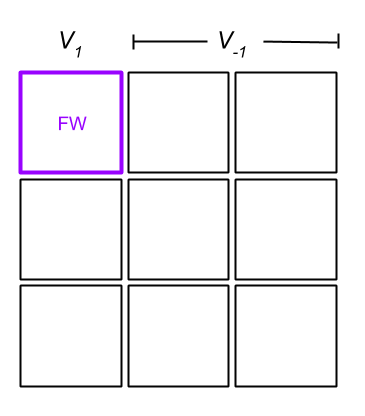
\includegraphics[scale = 0.3, trim = 0in -0.55in 0in 0in, clip]{blockApsp-2.png} &
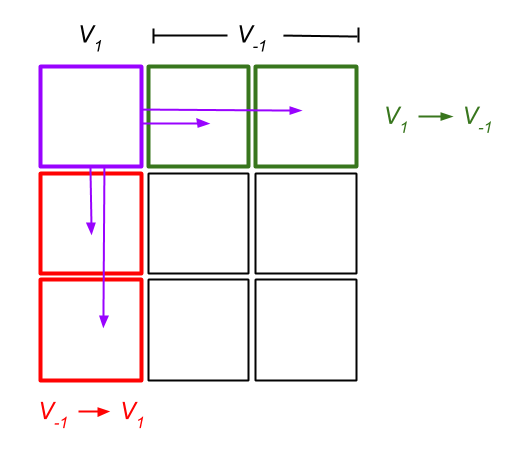
\includegraphics[scale = 0.3]{blockApsp-3.png} &
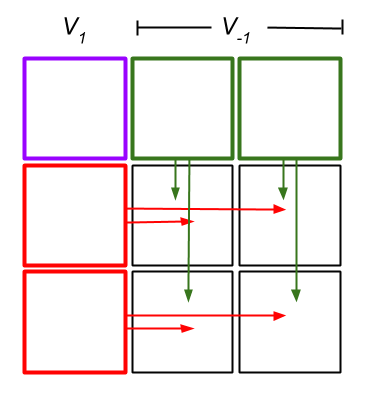
\includegraphics[scale = 0.3, trim = 0in -0.55in 0in 0in, clip]{blockApsp-4.png}\\
A-step & B-step & C-step
\end{tabular}
\end{figure}


\subsection{A-step}

In the $k$th iteration, the A-step is written in shorthand as
$S^{kk(k)} \leftarrow \text{APSP}(S^{kk(k-1)})$.  In fact, the updated
{\tt BlockMatrix} $S^{(k)}$ is not formed until the end of the C-step,
and in the A-step $S^{kk(k)}$ only exists on the driver.
The detailed A-step is as follows:
\begin{enumerate}
\item The block $S^{kk(k-1)}$ is copied to the driver via invoking the {\tt lookup} method with key $(k, k)$ on the {\tt  BlockMatrix} $S^{(k-1)}$
\item The driver locally computes $S^{kk(k)} \leftarrow \text{APSP}(S^{kk(k-1)})$
\end{enumerate}

\emph{Computation.} Only the driver performs computation, running
Floyd-Warshall on $S^{kk(k-1)}$.  This costs $\kappa_F b^3$.

\emph{Bandwidth.}
The lookup involves a one-to-one communication between the worker holding $S^{kk}$ and the driver.
Exactly $b^2$ words are transmitted.

\emph{Runtime.}
The runtime consists of the time taken to transmit $S^{kk}$ and the time to compute $\text{APSP}S^{kk}$.
Therefore the total runtime is
\[
\kappa_T b^2 + \kappa_F b^3
\]

\subsection{B-step}
In the $k$th iteration, the B-step is written in shorthand as
 $S^{kj(k)} \leftarrow \min(S^{kj(k-1)}, S^{kk(k)} \otimes S^{kj(k-1)})$ 
and 
$S^{ik(k)} \leftarrow \min(S^{ik(k-1)}, S^{ik(k-1)} \otimes S^{kk(k)})$
 in parallel.
This is accomplished by the following:
\begin{enumerate}
\item Form the RDD {\tt rows} and the RDD {\tt columns} by invoking
  the {\tt filter} method on $S^{(k-1)}$ to keep only the blocks
  $S^{ik(k-1)}$ and $S^{kj(k-1)}$ for $i = 1,\hdots, \ell$ and $j =
  1,\hdots, \ell$.
\item Broadcast $S^{kk(k)}$ from the driver to each worker holding a
  block in {\tt rows} or {\tt columns}.  There should be $\sqrt{p}$
  workers storing blocks in {\tt rows} and another $\sqrt{p}$ workers
  storing blocks in {\tt columns}.
\item Invoke {\tt mapValues} on {\tt rows} to perform the update
  $S^{kj(k)} \leftarrow \min(S^{kj(k-1)}, S^{kk(k)} \otimes S^{kj(k-1)})$ and similarly
  on {\tt cols} to perform the update $S^{ik(k)} \leftarrow \min(S^{ik(k-1)}, S^{ik(k-1)}
  \otimes S^{kk(k)})$
\end{enumerate}

\emph{Computation.}  Only the workers holding values in {\tt rows} or
     {\tt columns} perform computation, when {\tt mapValues} is
     invoked.  Each of those workers holds $\frac{n}{\sqrt{p}b}$
     blocks.  The update for each block entails a matrix multiplication
     costing $\kappa_M b^3$, so the cost per worker is $\kappa_m
     \frac{nb^2}{\sqrt{p}}$, and the total cost is $2\kappa_M b^2 n$.

\emph{Bandwidth.} The {\tt broadcast} step entails sending a $b \times
b$ matrix from the driver to $2\sqrt{p}$ workers.  Therefore the
bandwidth is $2\sqrt{p}b^2$

\emph{Runtime.} The runtime cost of the broadcast is
\[
\log(p)(\kappa_T b^2)
\]
due to bittorrent broadcast.
The runtime cost of computation is
\[
\kappa_M \frac{b^2 n}{\sqrt{p}}
\]
since each worker computes in parallel.
Hence the total runtime is
\[
\log(p)\kappa_T b^2 + \kappa_M \frac{b^2 n}{\sqrt{p}}
\]

\subsection{C-step}

In shorthand, the C-step is written as $S^{ij(k)} \leftarrow \min(S^{ij(k-1)}, S^{ik(k)} \otimes S^{kj(k)})$.
Here it becomes important to note the partitioner used for the various RDDs.
We assume that the same partitioner is used for all $S^{(0)}, \hdots, S^{(\ell)}$
and for the RDDs {\tt dupRows}, {\tt dupCols}, and {\tt temp} to be defined in the following.

\begin{enumerate}
\item Create RDD {\tt dupRows} by invoking {\tt flatMap} on {\tt rows} to flatMap the key-value pair
\[
(i, j, S^{ij})
\]
to the key-value pairs
\[
(1, j, S^{ij}), \hdots, (\ell, j, S^{ij})
\]
\item Create RDD {\tt dupCols} in an analogous way
\item Create RDD {\tt temp} by joining {\tt dupCols}, {\tt dupRows},
  and $S^{(k-1)}$.  The order of joining does not matter.
\item Create {\tt BlockMatrix} $S^{(k)}$ by invoking {\tt mapValues}
  to {\tt temp}.  The $(i, j)$ entry of {\tt temp} contains the blocks
  $S^{ij(k-1)}, S^{ik(k)}, S^{kj(k)}$ produced in the A-step and
  B-step.  The effect of {\tt mapValues} is to produce
\[
S^{ij(k)} \leftarrow \min(S^{ik(k-1)}, S^{ik(k)} \otimes S^{kj(k)})
\]
as $(i, j)$ block in $S^{(k)}$.
\end{enumerate}

\emph{Computation.}  The computation occurs when {\tt mapValues} is
called.  There, each worker computes $S^{ij(k)} \leftarrow
\min(S^{ik(k-1)}, S^{ik(k)} \otimes S^{kj(k)})$ for each of its
$n^2/(b^2 p)$ blocks.  The computation per block is $\kappa_M b^3$, and
hence the computation per worker is $\kappa_M \frac{n^2b}{p}$.
The total computational cost is $\kappa_M n^2b$.

\emph{Bandwidth.} Creation of {\tt dupRows} and {\tt dupCols} require
bandwidth.  Creation of {\tt temp} and $S^{(k)}$ do not require
bandwidth because of the map-side join.  Each block in {\tt rows} and
{\tt cols} must be sent to $\sqrt{p}$ workers.
Hence the bandwidth cost is $2 n b \sqrt{p}$.

\emph{Runtime.}  Creation of {\tt dupRows} requires each worker
holding values in {\tt rows} to transmit a message of size
$\frac{nb}{\sqrt{p}}$ to $\sqrt{p}$ other workers.  This must be done
sequentially under the current version of Spark (1.3.1) and hence
takes time
\[
\kappa_T nb
\]
In practice, the RDD {\tt dupRows} may be realized simultaneously.
However, since we do not analyze scheduling, we make the simplifying
assumption that {\tt dupRows} is created after {\tt dupCols} is
realized.
Therefore, the runtime due to communication-related issues is
\[
2\kappa_T nb
\]

Adding the computation per worker, the total runtime is
\[
2\kappa_T nb + \kappa_M \frac{n^2b}{p}
\]

\subsection{Latency-Free Totals}

We add up the costs derived for each step, and multiply by the number of iterations $\ell = n/b$.

\emph{Computational cost}:
\[
\kappa_M n^3 + 2\kappa_M n^2 b + \kappa_F n b^2
\]

\emph{Bandwidth}:
\[
2n^2 \sqrt{p} + 2n \sqrt{p} b + nb
\]

\emph{Runtime}:
\[
\kappa_M \frac{n^3}{p} + \kappa_M \frac{bn^2}{\sqrt{p}} + 2\kappa_T n^2 + \kappa_F nb^2 + (\log(p) + 1)\kappa_T nb
\]

\subsection{Latency-Added Analysis}

Here we \emph{uniform} network topology so the latency of transmission
is the same for every pair of workers.  This is in contrast to the
\emph{grid} or \emph{hypercube} topologies considered in most of the
existing literature on distributed APSP.

Here we will consider large-$p$ asymptotics so that that analysis is
not sensitive to the distribution of the lag, as long as has
exponential tails.

We assume the following model for latency:
\begin{itemize}
\item Whenever a machine transmits a message to another machine, it
  must wait a random amount of time $T$ to make contact with the
  recipient.  After contact is made, data is transferred at the rate
  $\frac{1}{\kappa_T}$.
\item The lags $T$ are independent and identically distributed.
For i.i.d. lags $T_i$ we have
\[
\text{E} \sup_{i=1}^p T_i = \kappa_L \log p
\]
where $\kappa_L$ is some constant.
\item \emph{Checkpointing:} Writing $m$ bytes to disk takes $\kappa_C
  m$ runtime and does not cost bandwidth nor CPU.
\end{itemize}

As a consequence of these assumptions, one-to-one communications incur
zero additional runtime due to lag, one-to-all (broadcast)
communications incur $\kappa_L \log^2 p$ additional runtime due to
lag and all-to-all communications incur $p \kappa_L \log(p)$ additional
runtime due to lag.

Given that the algorithm involves one one-to-one communication, one
one-to-all communication, four all-to-all communications, and $1/q$
checkpointing operations per iteration, the added runtime from latency
and checkpointing is
\[
L = \kappa_L(\log^2(p) + 4p\log(p)) + \kappa_C \frac{n^2}{pq}
\]

The runtime of the algorithm is given by
\[
L\frac{n}{b} + \kappa_M \frac{n^3}{p} + \kappa_M \frac{bn^2}{\sqrt{p}} + 2\kappa_T n^2 + \kappa_F nb^2 + (\log(p) + 1)\kappa_T nb
\]


\section{Correctness}

\subsection{Notation}

We assume a complete weighted and directed graph (with all possible
arcs).  Any incomplete graph is equivalent to the complete graph
where missing edges are represented by infinite-weight edges.

\begin{itemize}
\item If $i, j \in V$, let $i \to j$ denote the arc from $i$ to $j$.  An arc is also a path (of length 1).
\item If $v_1, \hdots, v_m \in V$, then $p = v_1\to \cdots \to v_m$  denotes a path composed of arcs $v_1 \to v_2, \hdots, v_{m-1} \to v_m$.
\item Let $w(p)$ denote the weight of the path, i.e. the weight of the arcs in the path
\item If $P$ is a set of paths, and $v \in V$, then
\[
v \to P = \{v \to p: p \in P\}
\]
and
\[
P \to v = \{p \to v: p \in P\}
\]
\item If $v, w \in V$ and $S \subset V$, then
\[ v \to S \to w = \{v \to s \to w: s \in S\}\]
and
\[
v \to S^* \to w = \{v \to w\} \cup \{v \to s_1 \to w: s \in S\} \cup \{v \to s_1 \to s_2 \to w: s_1, s_2 \in S\} \cup \cdots
\]
\item If $P$ is a set of paths,
\[
w(P) = \min_{p \in P} w(p)
\]
\item If $v, w \in V$, and $S, U \subset V$, then
\begin{align*}
v \to (S \to U \to S)^* \to w &= \{v \to w\} \cup \{v \to s_1 \to u \to s_2 \to w\} \cup \cdots\\
&= v \to (S \cup U)^* \to w
\end{align*}
\end{itemize}

It follows that the APSP matrix $S$ has the property
\[
S_{ij} = w(i \to V^* \to j)
\]

\subsection{Shortest paths and min-plus multiplication}

We review some basic principles linking shortest-path computations and min-plus multiplication which we will use in the proof.

Let $G$ be a graph with vertices $V = V_1 \cup V_2 \cup V_3$.
Let $H$ denote a matrix with $H_{ij} = w(i \to j)$ for $i \in V_1, j \in V_2$.
Let $I$ denote a matrix with $I_{jk} = w(j \to k)$ for $j \in V_2, k \in V_3$.
Then it follows that if $M = H \otimes I$,
\[
M_{ik} = w(i \to V_2 \to k)
\]
for $i \in V_1$ and $k \in V_3$.
Furthermore, suppose $L$ is a matrix with $L_{ik} = w(i \to k)$ for $i \in V_1$ and $k \in V_3$.
Then
\[
(\min(M, L))_{ik} = w((i \to k) \cup (i \to V_2 \to k))
\]
for $i \in V_1$ and $k \in V_3$.

Let $A$ be the adjacency matrix of $G$.
Define $A^2 = A \otimes A$ and $A^k = A^{k-1} \otimes A$.
We have
\[
(A^2)_{ij} = w(i \to V \to j)
\]
Note that a path $i \to i \to j$ or $i \to j \to j$ collapses to $i \to j$
since $A_{ii} = A_{jj} = 0$.
Also note that $\text{APSP}(A) = A^\infty$.
Therefore
\[
(\text{APSP}(A))_{ij} = (A^\infty)_{ij} = w(i \to V^* \to j)
\]


\subsection{Proof}

Let $V = V_1 \cup \cdots \cup V_\ell$ where $V_i = \{(b(i-1) + 1, \cdots, bi\}$.
Let $W_i = \bigcup_{k=1}^i V_i$, where $W_0 = \emptyset$.
Correctness follows if we can show that for $k = 0,\hdots, \ell$, we have
\[
S^{(k)}_{ij} = w(i \to W_k^* \to j)
\]
Fix $\ell$. We proceed by finite induction on $k$.

\emph{Base case.}

Recall that $S^{(0)} = A$.
Then
\[
S^{(0)}_{ij} = A_{ij} = w(i \to j) = w(i \to \emptyset^* \to j)
\]
so the base case $k=0$ is established.


\emph{Induction.}

Assume
\[
S^{(k-1)}_{ab} = w(a \to W_{k-1}^* \to b)
\]
Then in the $k$th iteration, the A-step computes
$S^{kk(k)} \leftarrow \text{APSP}(S^{kk(k-1)})$.
Thus we have
\[
S^{kk(k)}_{ab} = w(a \to (W_{k-1}^* \to V_k^* \to W_{k-1}^*)^* \to b) = w(a \to W_k^* \to b)
\]
From the B-step we have
 $S^{kj(k)} \leftarrow \min(S^{kj(k-1)}, S^{kk(k)} \otimes S^{kj(k-1)})$ 
and 
$S^{ik(k)} \leftarrow \min(S^{ik(k-1)}, S^{ik(k)} \otimes S^{kk(k)})$.
Therefore,
\begin{align*}
S^{ik(k)}_{ab} &= w((a \to W_{k-1}^* \to b) \cup (a \to W_k^* \to V_k \to W_{k-1}^* \to b))\\
&= w(a \to W_k^* \to b)
\end{align*}
and similarly
\[
S^{ki(k)}_{ab} = w(a \to W_k^* \to b)
\]
Therefore in the C-step, which computes
$S^{ij(k)} \leftarrow \min(S^{ij(k-1)}, S^{ik(k)} \otimes S^{kj(k)})$,
we have
\begin{align*}
S^{ij(k)}_{ab} &= w((a \to W_{k-1}^* \to b) \cup (a \to W_k^* \to V_k \to W_k^* \to b))\\
&= w(a \to W_k^* \to b)
\end{align*}
Hence we have shown
\[
S^{(k)}_{ab} = w(a \to W_k^* \to b)
\]
as needed.

\section{Results}
To implement the algorithm in Spark, we take use of
the BlockMatrix class in Mllib. The two main operations
in our algorithm: $\min(A, B)$ and $A \otimes B$ of matrices
$A$ and $B$ are analogous to the ``add'' and ``multiply''
operations of matrices. Thus, we also use the Grid Partitioner defined in the BlockMatrix class to avoid 
unnecessary shuffling of data in these operations.
As how people build the BlockMatrix class, our local matrix operations $\min(A, B)$ and $A \otimes B$
are also done via the breeze matrix operations.

The other technique we use is checkpointing. In each iteration, we are updating the whole $n \times n$ shortest paths matrix, which is stored as an RDD. Thus, we keep
generating new RDDs depending on RDDs of previous iterations, which causes the length of the dependency chain to keep increasing with the number of iterations.
By checkpointing, RDD can be saved to disk and the lineage of RDDs can be truncated. We checkpoint the RDDs
every 20 iterations following Meng and Das (2014)'s comments. 

We run the algorithm for $n = 500$ and $n = 1000$ 
on a local computer with $4$ cores and $8$GB memories in 
total. Thus, $p = 4$ which is also the total number of partitions. Figure \ref{fig:time-result} shows the total
run time for different block sizes. The use of blocks reduces the run time of distributed Floyd-Warshall substantially. The optimal block size $b$ depends on the trade-off of reduced latency time and the extra computation time. In our experiment, for both $n = 500$
and $n = 1000$, $b = 250$ performs the best among all the
choices.

\begin{figure}[ht]
\centering
\begin{subfigure}[b]{0.45\textwidth}
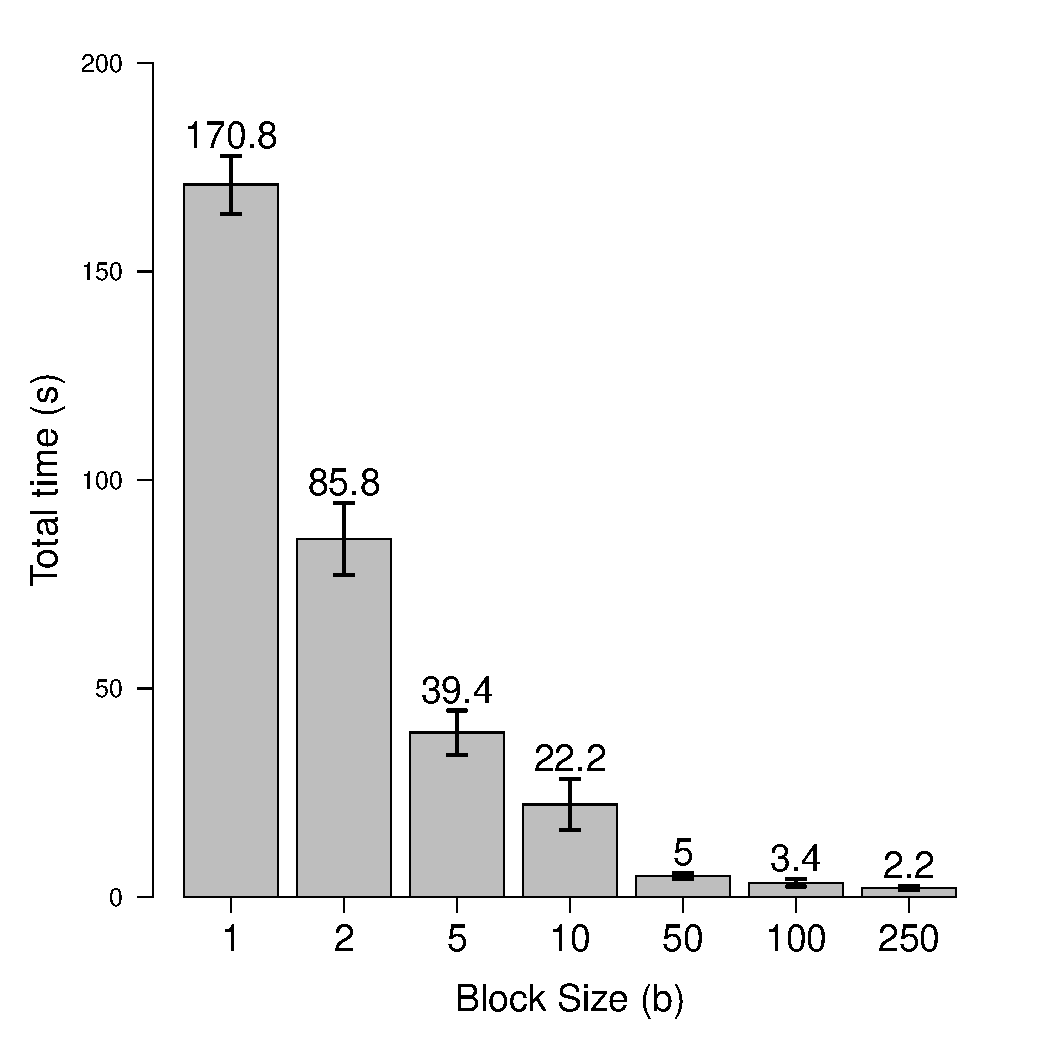
\includegraphics[width = \textwidth]{time.pdf}
\caption{n = 500}
\end{subfigure}
\begin{subfigure}[b]{0.45\textwidth}
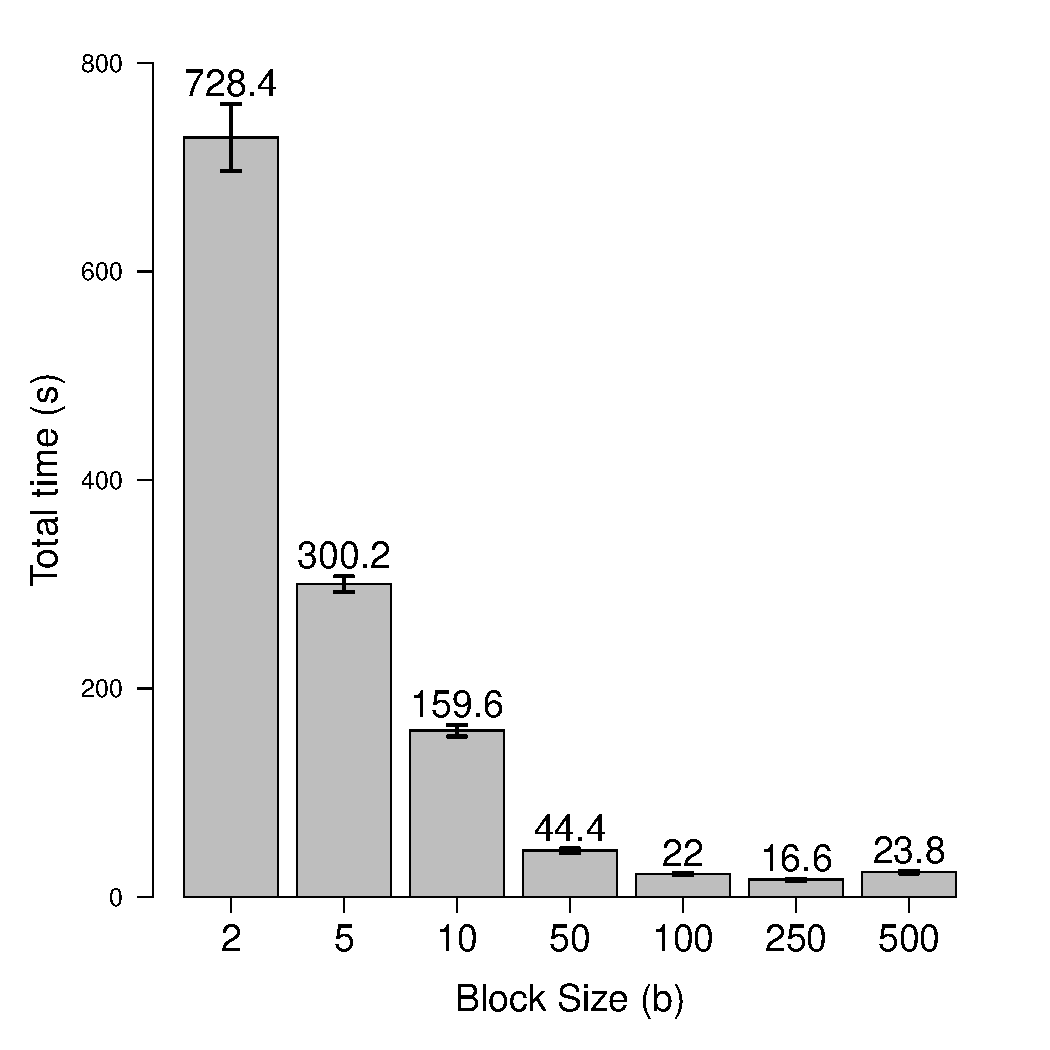
\includegraphics[width = \textwidth]{time1000.pdf}
\caption{n = 1000}
\end{subfigure}
\caption{The total run time versus the block size: the total run time is in seconds. The error bars are the standard deviations of $5$ random runs.}
\label{fig:time-result}
\end{figure}

The code is publicly available at {\tt https://github.com/arzavj/spark-all-pairs-shortest-path}.

\section{References}
\begin{itemize}
\item Buluc, Aydın, John R. Gilbert, and Ceren Budak. "Solving path problems on the GPU." Parallel Computing 36.5 (2010): 241-253.
\item Zaharia, M., \& Chowdhury, M. (2010). Spark: cluster computing with working sets.
\item Kumar, V., \& Singh, V. (1991). Scalability of parallel algorithms for the all-pairs shortest-path problem. Journal of Parallel and Distributed Computing, 13(2), 124–138. doi:10.1016/0743-7315(91)90083-L
\item Solomonik, E., Buluc, A., \& Demmel, J. (2013). Minimizing communication in all-pairs shortest paths. Proceedings - IEEE 27th International Parallel and Distributed Processing Symposium, IPDPS 2013, 548–559. doi:10.1109/IPDPS.2013.111
\item Meng, Xiangrui \& Das, Tathagata (2014). Re: java.lang.StackOverflowError when calling count(). Retrived from http://apache-spark-user-list.1001560.n3.nabble.com/java-lang-StackOverflowError-when-calling-count-td5649.html
\item Jain, Arzav,. Wang, Jingshu., Zheng, Charles. spark-all-pairs-shortest-path. 
{\tt https://github.com/arzavj/spark-all-pairs-shortest-path}
\end{itemize}


\end{document}